\documentclass{beamer}
\usepackage{tikz}
\usetikzlibrary{shapes,arrows,positioning,fit,backgrounds}

\usetheme{Madrid}
\usecolortheme{whale}

\usepackage{listings}

\setbeamertemplate{navigation symbols}{}

\title{Introduction to Mobile Computing and App Development}
\subtitle{Lecture 1: Foundations for Beginners}
\author{Brendan Shea, PhD}
\date{Intro to Mobile Apps}

\begin{document}
	
	\begin{frame}
		\titlepage
	\end{frame}
	
	\begin{frame}
		\frametitle{What Are Mobile Devices? Understanding Today's Mobile Landscape}
		
		\begin{itemize}
			\item \textbf{Mobile devices} are portable computing devices designed for use while on the move, including smartphones, tablets, smartwatches, and other wearable technology.
			\item Mobile devices typically feature touch screens, wireless connectivity, and compact form factors that prioritize portability over raw computing power.
			\item Most mobile devices run specialized operating systems (iOS, Android) that are optimized for touch interaction, battery efficiency, and mobile-specific tasks.
			\item The global mobile ecosystem now connects billions of users, creating unprecedented opportunities for app developers to reach wide audiences.
		\end{itemize}
		
		\begin{alertblock}{Key Insight}
			\scriptsize
			Mobile devices represent a fundamentally different computing paradigm compared to traditional desktop computers, requiring developers to rethink how users interact with technology.
		\end{alertblock}
		
	\end{frame}
	
	\begin{frame}
		\frametitle{How Mobile Computing Differs from Desktop Computing}
		
		\begin{itemize}
			\item Mobile computing prioritizes \textbf{contextual awareness}, using sensors and location data to deliver experiences tailored to the user's current situation and environment.
			\item Unlike desktop computers with consistent power sources, mobile devices operate under strict \textbf{resource constraints} including battery life, processing power, memory, and network connectivity.
			\item Mobile interfaces employ \textbf{touch-centric design patterns} that replace traditional mouse and keyboard interactions with gestures, taps, and on-screen keyboards.
			\item Mobile apps typically focus on performing specific tasks very well, rather than the multi-purpose functionality common in desktop software.
		\end{itemize}
		
		\begin{columns}[t]
			\scriptsize
			\column{.45\textwidth}
			\textbf{Desktop Computing}
			\begin{itemize}
				\item Stationary usage
				\item Consistent power source
				\item Large displays
				\item Keyboard \& mouse input
				\item Extended usage sessions
			\end{itemize}
			
			\column{.45\textwidth}
			\textbf{Mobile Computing}
			\begin{itemize}
				\item On-the-go usage
				\item Battery dependency
				\item Small touchscreens
				\item Touch \& gesture input
				\item Brief interaction sessions
			\end{itemize}
		\end{columns}
		
	\end{frame}
	
	\begin{frame}
		\frametitle{The Evolution of Mobile Technology: From Brick Phones to Smartphones}
		
		\begin{itemize}
			\item The journey began with basic cellular phones or \textbf{"feature phones"} that primarily handled voice calls and eventually simple text messaging.
			\item Early \textbf{PDAs} (Personal Digital Assistants) like the Palm Pilot introduced touchscreens and basic applications but lacked cellular connectivity.
			\item The 2007 introduction of the iPhone marked a pivotal moment, combining phone functionality with internet access and a revolutionary touch interface in a single device.
			\item Modern smartphones now function as powerful computers, featuring advanced processors, high-resolution displays, sophisticated sensors, and app ecosystems that enable countless functions.
		\end{itemize}
		
		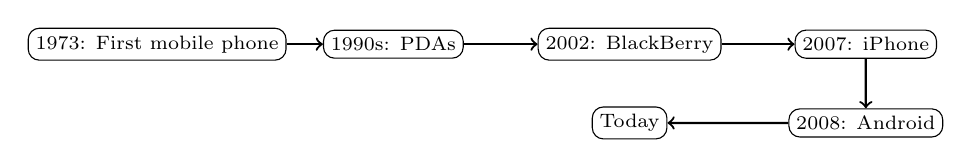
\begin{tikzpicture}[node distance=1cm, scale = 0.7]
			\scriptsize
			\node (start) [draw, rounded corners] {1973: First mobile phone};
			\node (pda) [draw, rounded corners, right of=start, xshift=2cm] {1990s: PDAs};
			\node (bb) [draw, rounded corners, right of=pda, xshift=2cm] {2002: BlackBerry};
			\node (iphone) [draw, rounded corners, right of=bb, xshift=2cm] {2007: iPhone};
			\node (android) [draw, rounded corners, below of=iphone] {2008: Android};
			\node (today) [draw, rounded corners, left of=android, xshift=-2cm] {Today};
			
			\draw[thick,->] (start) -- (pda);
			\draw[thick,->] (pda) -- (bb);
			\draw[thick,->] (bb) -- (iphone);
			\draw[thick,->] (iphone) -- (android);
			\draw[thick,->] (android) -- (today);
		\end{tikzpicture}
		
	\end{frame}
	
	\begin{frame}[fragile]
		\frametitle{Mobile Device Capabilities: Hardware Components That Enable Apps}
		
		\begin{itemize}
			\item Modern mobile devices include \textbf{sensors} like accelerometers, gyroscopes, and GPS that allow apps to respond to movement, orientation, and location.
			\item \textbf{Communication hardware} (cellular radios, Wi-Fi, Bluetooth, NFC) enables connectivity with networks, other devices, and physical objects like payment terminals.
			\item High-resolution \textbf{cameras} and microphones serve as data collection tools that apps can leverage for photography, augmented reality, voice recognition, and more.
			\item System-on-chip (SoC) designs integrate \textbf{processors}, graphics, memory, and specialized hardware for machine learning and image processing into efficient packages.
		\end{itemize}
		
	\end{frame}
	
	\begin{frame}
		\frametitle{The Mobile Operating System Ecosystem: iOS, Android, and Others}
		
		\begin{itemize}
			\item \textbf{iOS} is Apple's proprietary operating system that runs exclusively on Apple hardware like iPhones and iPads, offering tight integration, consistent user experience, and advanced security features.
			\item \textbf{Android}, developed by Google, is an open-source operating system that powers the majority of non-Apple mobile devices, providing more customization options and running on hardware from many manufacturers.
			\item Mobile operating systems manage device hardware, provide standardized programming interfaces for apps, and facilitate app distribution through official stores.
		\end{itemize}
		
		\begin{block}{\scriptsize{Market Share Comparison (2024)}}
			\scriptsize{
				\begin{tabular}{|l|c|l|}
					\hline
					\textbf{OS} & \textbf{\% of Market} & \textbf{Key Characteristics} \\
					\hline
					Android & $\sim$70\% & Open-source, diverse hardware, customizable \\
					\hline
					iOS & $\sim$29\% & Closed ecosystem, premium hardware, privacy focus \\
					\hline
					Others & $\sim$1\% & Regional focus, specialized use cases \\
					\hline
				\end{tabular}
			}
		\end{block}
		
	\end{frame}
	
	\begin{frame}
		\frametitle{How Users Interact with Mobile Devices: Touch, Voice, and Sensors}
		
		\begin{itemize}
			\item \textbf{Touch-based interaction} is the primary interface for mobile devices, with users performing gestures like tapping, swiping, pinching, and long-pressing to control applications.
			\item \textbf{Voice commands} have become increasingly important, with virtual assistants like Siri, Google Assistant, and Alexa allowing hands-free control of devices and applications.
			\item Modern mobile devices incorporate numerous \textbf{sensors} that enable context-aware applications, including accelerometers for motion detection, light sensors for screen brightness, and proximity sensors for call handling.
		\end{itemize}
		
		
	\end{frame}
	
	\begin{frame}
		\frametitle{What Exactly Is a Mobile App?}
		
		\begin{itemize}
			\item A \textbf{mobile application} (or "app") is a software program designed specifically to run on mobile devices, optimized for their screen sizes, hardware capabilities, and usage patterns.
			\item Unlike desktop software, mobile apps typically focus on performing a limited set of functions very well, with interfaces designed for quick, focused interactions rather than extended use sessions.
			\item Apps access device hardware through \textbf{APIs} (Application Programming Interfaces) provided by the operating system, allowing them to use cameras, location services, and other device features.
		\end{itemize}
		
		\begin{exampleblock}{\scriptsize{Examples of Different App Categories}}
			\scriptsize{
				\begin{itemize}
					\item \textbf{Utility apps:} Calculators, weather, calendars - solving practical everyday problems
					\item \textbf{Social apps:} Instagram, TikTok, WhatsApp - connecting people digitally
					\item \textbf{Entertainment apps:} Games, streaming services - providing leisure activities
					\item \textbf{Productivity apps:} Document editors, note-taking tools - enhancing work efficiency
				\end{itemize}
			}
		\end{exampleblock}
		
	\end{frame}
	
	\begin{frame}
		\frametitle{The App Store Phenomenon: How Apps Are Distributed}
		
		\begin{itemize}
			\small
			\item \textbf{App stores} are centralized digital marketplaces where users discover, download, and update mobile applications, with the Apple App Store and Google Play Store being the two dominant platforms.
			\item App stores provide important \textbf{security benefits} by reviewing apps for malicious code, setting quality standards, and enabling quick removal of problematic applications.
			\item For developers, app stores offer a \textbf{distribution channel} with built-in payment processing, user reviews, analytics, and the potential to reach millions of users globally.
		\end{itemize}
		
		\scriptsize{
			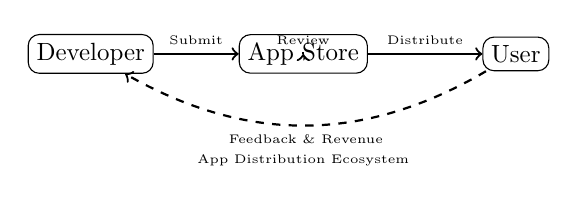
\begin{tikzpicture}[scale=0.9, transform shape, every node/.style={rectangle, rounded corners, draw}]
				\node (dev) at (0,0) {Developer};
				\node (store) at (3,0) {App Store};
				\node (user) at (6,0) {User};
				
				\draw[->, thick] (dev) -- node[above, draw=none] {\tiny{Submit}} (store);
				\draw[->, thick] (store) -- node[above, draw=none] {\tiny{Review}} (store);
				\draw[->, thick] (store) -- node[above, draw=none] {\tiny{Distribute}} (user);
				\draw[->, thick, dashed] (user) to[bend left] node[below, draw=none] {\tiny{Feedback \& Revenue}} (dev);
				
				\node[draw=none] at (3,-1.5) {\tiny{App Distribution Ecosystem}};
			\end{tikzpicture}
		}
		
	\end{frame}
	
	\begin{frame}
		\frametitle{Native Apps Explained: Built for Specific Platforms}
		
		\begin{itemize}
			\item \textbf{Native apps} are applications developed specifically for a single operating system (iOS or Android) using the platform's standard programming languages and development tools.
			\item Native apps can fully access all device hardware and platform-specific features, resulting in optimal performance, seamless integration with the operating system, and familiar user interface patterns.
			\item The main drawback of native development is that separate codebases must be maintained for each platform, increasing development time and cost.
		\end{itemize}
		
		\begin{alertblock}{\scriptsize{Native App Advantages}}
			\scriptsize{
				\begin{itemize}
					\item Maximum performance and responsiveness
					\item Full access to all platform APIs and hardware features
					\item Platform-specific user interface that feels natural to users
					\item Better discoverability in app stores
				\end{itemize}
			}
		\end{alertblock}
		
	\end{frame}
	
	\begin{frame}
		\frametitle{Web Apps Explained: Mobile-Optimized Websites}
		
		\begin{itemize}
			\item \textbf{Web apps} are essentially websites optimized for mobile devices, built using standard web technologies (HTML, CSS, JavaScript) and accessed through a mobile browser rather than being installed from an app store.
			\item Modern web apps use \textbf{responsive design} techniques to adapt their layouts and functionality to different screen sizes and orientations.
			\item The key advantage of web apps is their cross-platform compatibility—they can run on any device with a web browser without requiring separate development for each platform.
			\item Web apps have limited access to device hardware and features compared to native apps, and typically cannot function offline without special techniques.
		\end{itemize}
		
		\begin{center}
			\scriptsize{
				\begin{tabular}{|p{4cm}|p{4cm}|}
					\hline
					\textbf{Advantages} & \textbf{Limitations} \\
					\hline
					Single codebase for all platforms & Limited hardware access \\
					No installation required & Requires internet connection \\
					Instantly updated for all users & Lower performance than native \\
					No app store approval process & Cannot be listed in app stores \\
					\hline
				\end{tabular}
			}
		\end{center}
		
	\end{frame}
	
	\begin{frame}
		\frametitle{Hybrid Apps Explained: Blending Native and Web Approaches}
		
		\begin{itemize}
			\item \textbf{Hybrid apps} combine elements of both native and web apps by wrapping web technologies (HTML, CSS, JavaScript) inside a native container that can be installed from app stores.
			\item Hybrid apps offer a "write once, run anywhere" approach that reduces development time and cost compared to maintaining separate native codebases for each platform.
			\item While performance has improved significantly, hybrid apps may still lag behind native apps for graphics-intensive applications or those requiring complex device integrations.
		\end{itemize}
		
		\scriptsize{
			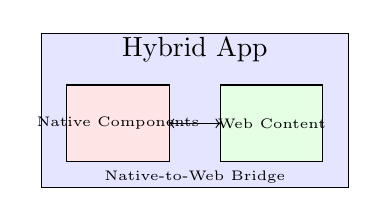
\begin{tikzpicture}[scale=0.65]
				\draw[fill=blue!10] (0,0) rectangle (6,3);
				\node at (3,2.7) {Hybrid App};
				
				\draw[fill=red!10] (0.5,0.5) rectangle (2.5,2);
				\node[align=center] at (1.5,1.25) {\tiny{Native Components}};
				
				\draw[fill=green!10] (3.5,0.5) rectangle (5.5,2);
				\node[align=center] at (4.5,1.25) {\tiny{Web Content}};
				
				\draw[<->] (2.5,1.25) -- (3.5,1.25);
				
				\node[align=center] at (3,0.2) {\tiny{Native-to-Web Bridge}};
			\end{tikzpicture}
		}
	\end{frame}
	
	\begin{frame}
		\frametitle{PWAs (Progressive Web Apps): The Best of Both Worlds?}
		
		\begin{itemize}
			\item \textbf{Progressive Web Apps (PWAs)} are web applications that use modern web capabilities to provide an app-like experience, including offline functionality, push notifications, and home screen installation.
			\item PWAs use \textbf{service workers} (JavaScript files that run separately from the web page) to cache content and enable offline access, solving a major limitation of traditional web apps.
			\item Unlike hybrid apps that use platform-specific containers, PWAs are truly cross-platform and update automatically when users access them, eliminating the app store update process.
			\item Major companies like Twitter, Spotify, and Pinterest have adopted PWAs to provide consistent experiences across devices while reducing development and maintenance costs.
		\end{itemize}
		
	\end{frame}
	
	\begin{frame}
		\frametitle{The Mobile App Development Lifecycle: From Idea to Launch}
		
		\begin{itemize}
			\item The mobile app development process begins with \textbf{ideation and planning}, where developers define the app's purpose, target audience, and key features, often creating wireframes and user stories.
			\item The \textbf{design phase} transforms concepts into visual mockups and user interface designs, considering platform conventions, accessibility guidelines, and brand identity.
			\item \textbf{Development} involves writing the actual code, integrating APIs, and building the application's frontend and backend components through iterative cycles.
			\item After thorough \textbf{testing}, the app is submitted to app stores for review, then marketed, monitored, and regularly updated based on user feedback and changing requirements.
		\end{itemize}
		
		\scriptsize{
			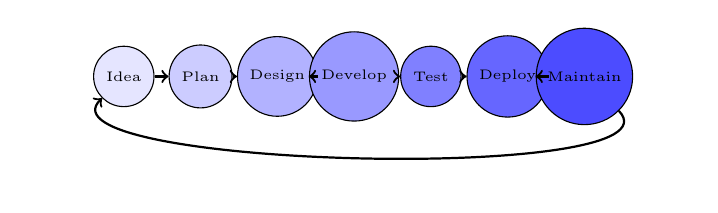
\begin{tikzpicture}[scale=0.65, node distance=1.2cm]
				\node[draw, circle, fill=blue!10] (idea) at (0,0) {\tiny{Idea}};
				\node[draw, circle, fill=blue!20] (plan) at (1.5,0) {\tiny{Plan}};
				\node[draw, circle, fill=blue!30] (design) at (3,0) {\tiny{Design}};
				\node[draw, circle, fill=blue!40] (dev) at (4.5,0) {\tiny{Develop}};
				\node[draw, circle, fill=blue!50] (test) at (6,0) {\tiny{Test}};
				\node[draw, circle, fill=blue!60] (deploy) at (7.5,0) {\tiny{Deploy}};
				\node[draw, circle, fill=blue!70] (maintain) at (9,0) {\tiny{Maintain}};
				
				\draw[->,thick] (idea) -- (plan);
				\draw[->,thick] (plan) -- (design);
				\draw[->,thick] (design) -- (dev);
				\draw[->,thick] (dev) -- (test);
				\draw[->,thick] (test) -- (deploy);
				\draw[->,thick] (deploy) -- (maintain);
				\draw[->,thick, bend left] (maintain) to[out=135, in=45, looseness=0.5] (idea);
			\end{tikzpicture}
		}
		
	\end{frame}
	
	\begin{frame}
		\frametitle{User-Centered Design: Why Mobile UX Is Critical}
		
		\begin{itemize}
			\item \textbf{User-Centered Design (UCD)} is a design philosophy that prioritizes users' needs, preferences, and limitations throughout the entire development process.
			\item Mobile users typically engage with apps in brief sessions (often less than 2 minutes), making intuitive interfaces and clear navigation essential for providing value quickly.
			\item Unlike desktop software where users might tolerate learning curves, mobile users typically abandon apps that are confusing or difficult to use, with studies showing that over 80\% of users never return after a poor first experience.
		\end{itemize}
		
		\begin{exampleblock}{\scriptsize{Key UX Design Principles for Mobile}}
			\scriptsize{
				\begin{itemize}
					\item \textbf{Thumb-friendly design:} Place important elements within easy reach of thumbs
					\item \textbf{Minimal input:} Reduce typing through autocomplete, selection lists, and defaults
					\item \textbf{Progressive disclosure:} Show only essential information first, reveal details on demand
					\item \textbf{Clear feedback:} Confirm actions and provide visual cues about system status
				\end{itemize}
			}
		\end{exampleblock}
		
	\end{frame}
	
	\begin{frame}
		\frametitle{Responsive Design: Adapting to Different Screen Sizes}
		
		\begin{itemize}
			\item \textbf{Responsive design} is an approach to creating interfaces that automatically adjust their layout, content, and functionality based on the screen size and orientation of the device.
			\item Mobile apps must function across a wide range of device sizes, from small phones (around 4 inches) to large tablets (12+ inches), with both portrait and landscape orientations.
			\item Responsive layouts typically use \textbf{flexible grids and containers} that resize proportionally rather than fixed pixel dimensions, often combined with breakpoints that trigger layout changes at specific screen widths.
		\end{itemize}
		
		\begin{center}
			\scriptsize{
				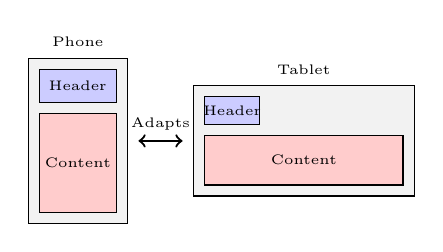
\begin{tikzpicture}[scale=0.7]
					% Phone in portrait
					\draw[fill=black!5] (0,0) rectangle (1.8,3);
					\draw[fill=blue!20] (0.2,2.2) rectangle (1.6,2.8);
					\draw[fill=red!20] (0.2,0.2) rectangle (1.6,2);
					
					% Tablet in landscape
					\draw[fill=black!5] (3,0.5) rectangle (7,2.5);
					\draw[fill=blue!20] (3.2,1.8) rectangle (4.2,2.3);
					\draw[fill=red!20] (3.2,0.7) rectangle (6.8,1.6);
					
					% Arrows
					\draw[<->, thick] (2,1.5) -- (2.8,1.5);
					
					% Labels
					\node at (0.9,3.3) {\tiny{Phone}};
					\node at (5,2.8) {\tiny{Tablet}};
					\node at (2.4,1.8) {\tiny{Adapts}};
					
					% Elements
					\node at (0.9,2.5) {\tiny{Header}};
					\node at (0.9,1.1) {\tiny{Content}};
					\node at (3.7,2.05) {\tiny{Header}};
					\node at (5,1.15) {\tiny{Content}};
				\end{tikzpicture}
			}
		\end{center}
		
	\end{frame}
	
	\begin{frame}
		\frametitle{Design Patterns in Mobile: Navigation Models That Users Expect}
		
		\begin{itemize}
			\item \textbf{Design patterns} are standardized solutions to common design problems that help create consistent, intuitive user experiences that feel familiar to users.
			\item Effective navigation makes the structure of the app immediately clear to users, allowing them to build an accurate mental model of where they are and where they can go.
		\end{itemize}
		
		\begin{block}{\scriptsize{Common Mobile Navigation Patterns}}
			\scriptsize{
				\begin{tabular}{|p{2.5cm}|p{4.5cm}|}
					\hline
					\textbf{Pattern} & \textbf{Best Used For} \\
					\hline
					Tab Bar/Bottom Navigation & 3-5 equally important sections \\
					\hline
					Hamburger Menu & Apps with many secondary sections \\
					\hline 
					Navigation Drawer & Content-heavy apps needing categorization \\
					\hline
					Gesture Navigation & Immersive experiences like games or media \\
					\hline
				\end{tabular}
			}
		\end{block}
		
	\end{frame}
	
	\begin{frame}
		\frametitle{Mobile App Architecture: Frontend and Backend Basics}
		
		\begin{itemize}
			\item \textbf{Frontend architecture} refers to the client-side portion of a mobile app that users directly interact with, including the user interface, local data storage, and device-specific functionality.
			\item \textbf{Backend architecture} encompasses server-side components that power an app, including databases, authentication systems, and business logic that works across all users of the application.
			\item Many modern mobile apps use a \textbf{client-server model}, where the app on the device (client) communicates with remote servers through APIs to retrieve or store data.
		\end{itemize}
		
		\begin{center}
			\scriptsize{
				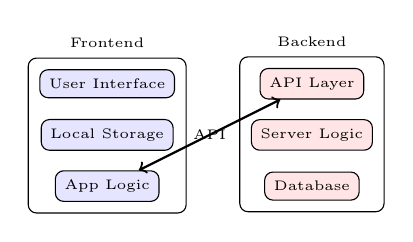
\begin{tikzpicture}[scale=0.65, every node/.style={rectangle, rounded corners=3pt, draw, align=center}]
					% Frontend
					\node[fill=blue!10] (ui) at (0,1) {\tiny{User Interface}};
					\node[fill=blue!10] (local) at (0,0) {\tiny{Local Storage}};
					\node[fill=blue!10] (logic) at (0,-1) {\tiny{App Logic}};
					
					% Backend
					\node[fill=red!10] (api) at (4,1) {\tiny{API Layer}};
					\node[fill=red!10] (server) at (4,0) {\tiny{Server Logic}};
					\node[fill=red!10] (db) at (4,-1) {\tiny{Database}};
					
					% Group boxes
					\node[rectangle, draw, fit=(ui) (local) (logic), inner sep=4pt, label=above:\tiny{Frontend}] {};
					\node[rectangle, draw, fit=(api) (server) (db), inner sep=4pt, label=above:\tiny{Backend}] {};
					
					% Connection
					\draw[<->, thick] (logic) -- node[midway, draw=none] {\tiny{API}} (api);
					
				\end{tikzpicture}
			}
		\end{center}
		
	\end{frame}
	
	\begin{frame}
		\frametitle{APIs: How Mobile Apps Communicate with Servers}
		
		\begin{itemize}
			\item \textbf{APIs} (Application Programming Interfaces) are sets of rules and protocols that allow different software components to communicate with each other, enabling mobile apps to request data or services from external systems.
			\item \textbf{RESTful APIs} are the most common type used in mobile development, organizing communications around resources (like users or products) that can be accessed through standard HTTP methods (GET, POST, PUT, DELETE).
			\item APIs typically transfer data in standardized formats like \textbf{JSON} (JavaScript Object Notation) or XML, which can be efficiently parsed by mobile applications regardless of the programming language used.
			\item Well-designed APIs include authentication mechanisms, rate limiting, and versioning to ensure security, reliability, and backward compatibility as both apps and servers evolve.
		\end{itemize}
			
	\end{frame}
	
	\begin{frame}
		\frametitle{Cross-Platform vs. Platform-Specific Development: Pros and Cons}
		
		\begin{itemize}
			\item \textbf{Platform-specific development} (native) means building separate apps for iOS and Android using their respective programming languages and tools, resulting in optimal performance and full access to platform features.
			\item \textbf{Cross-platform development} uses frameworks like Flutter, React Native, or Xamarin to write code once and deploy it to multiple platforms, reducing development time and maintenance costs.

		\end{itemize}
		
		\begin{alertblock}{\scriptsize{Decision Factors}}
			\scriptsize{
				\begin{tabular}{|p{4.5cm}|p{4.5cm}|}
					\hline
					\textbf{Choose Native When} & \textbf{Choose Cross-Platform When} \\
					\hline
					Maximum performance is critical & Time-to-market is the priority \\
					\hline
					Need deep platform integration & Limited budget or resources \\
					\hline
					Building platform-specific features & Building MVP or prototype \\
					\hline
					Have separate iOS/Android teams & Small team with web expertise \\
					\hline
				\end{tabular}
			}
		\end{alertblock}
		
	\end{frame}
	
	\begin{frame}
		\frametitle{Introduction to Flutter: A Modern Cross-Platform Framework}
		
		\begin{itemize}
			\item \textbf{Flutter} is Google's UI toolkit for building natively compiled applications for mobile, web, and desktop from a single codebase, using the \textbf{Dart} programming language.
			\item Unlike other cross-platform frameworks that use native components or web views, Flutter renders all UI elements using its own high-performance rendering engine, ensuring consistent appearance across platforms.
			\item Flutter's \textbf{widget-based architecture} makes UI development more intuitive—everything in Flutter is a widget, from buttons and text fields to layouts and animations.
		\end{itemize}
		
		\begin{center}
			\scriptsize{
				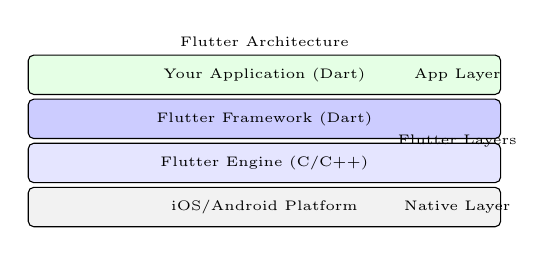
\begin{tikzpicture}[scale=0.7, every node/.style={draw, rectangle, rounded corners=2pt}]
					% Platform layers
					\node[fill=gray!10, minimum width=6cm, minimum height=0.5cm] at (3,0) {\tiny{iOS/Android Platform}};
					
					% Flutter layers
					\node[fill=blue!10, minimum width=6cm, minimum height=0.5cm] at (3,0.8) {\tiny{Flutter Engine (C/C++)}};
					\node[fill=blue!20, minimum width=6cm, minimum height=0.5cm] at (3,1.6) {\tiny{Flutter Framework (Dart)}};
					
					% App layer
					\node[fill=green!10, minimum width=6cm, minimum height=0.5cm] at (3,2.4) {\tiny{Your Application (Dart)}};
					
					% Labels
					\node[draw=none] at (6.5,0) {\tiny{Native Layer}};
					\node[draw=none] at (6.5,1.2) {\tiny{Flutter Layers}};
					\node[draw=none] at (6.5,2.4) {\tiny{App Layer}};
					
					% Title
					\node[draw=none] at (3,3) {\tiny{Flutter Architecture}};
				\end{tikzpicture}
			}
		\end{center}
		
	\end{frame}
	
	\begin{frame}
		\frametitle{Why Flutter Matters: Key Advantages for New Developers}
		
		\begin{itemize}
			\item Flutter's \textbf{hot reload} feature allows developers to see changes instantly without restarting the app, dramatically accelerating the development cycle and making it ideal for beginners learning through experimentation.
			\item The \textbf{single codebase} approach simplifies maintenance and ensures feature parity across platforms, eliminating the need to learn multiple programming languages and frameworks.
			\item Flutter has a \textbf{gentle learning curve}, especially for those with experience in object-oriented programming, and its comprehensive documentation includes many tutorials and examples specifically designed for beginners.
			\item The framework is backed by Google and has a rapidly growing \textbf{community}, providing beginners with abundant learning resources, third-party packages, and support forums.
		\end{itemize}
	\end{frame}
	
	\begin{frame}
		\frametitle{Dart Programming Language: The Foundation of Flutter}
		
		\begin{itemize}
			\item \textbf{Dart} is a client-optimized programming language created by Google that serves as Flutter's foundation, combining the productivity benefits of high-level languages with the performance characteristics needed for mobile development.
			\item Dart features a \textbf{C-style syntax} familiar to developers with experience in languages like Java, JavaScript, or C\#, making it relatively easy to learn for those with some programming background.
			\item The language is \textbf{strongly typed} but includes type inference, allowing developers to benefit from type safety without excessive verbosity in their code.
			\item Dart was specifically designed for building user interfaces, with features like an asynchronous programming model using \textbf{Futures} and \textbf{async/await} syntax that simplifies handling operations like network requests.
		\end{itemize}
	\end{frame}
	
	\begin{frame}[fragile]
		
		\frametitle{Sample Dart Code}

\scriptsize
		\begin{lstlisting}[language=Java]
// A simple Dart class
class User {
	final String name;
	final int age;
	
// Constructor
	User(this.name, this.age);

// Method
String greet() {
	return "Hello, my name is $name and I'm $age years old.";
}
}

// Using the class
void main() {
	var user = User("Alex", 25);
	print(user.greet());
}
		\end{lstlisting}
	\end{frame}
	
	\begin{frame}
		\frametitle{Understanding Widgets: The Building Blocks of Flutter Apps}
		
		\begin{itemize}
			\item In Flutter, \textbf{widgets} are the fundamental building blocks used to create user interfaces—everything from buttons and text to layouts and animations is a widget.
			\item Flutter uses a \textbf{composition-based} approach where complex interfaces are created by combining and nesting simpler widgets, forming a widget tree that represents the entire UI.
		\end{itemize}
		
		\begin{center}
			\scriptsize{
				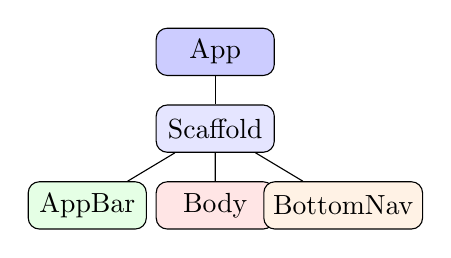
\begin{tikzpicture}[scale=0.65, 
					every node/.style={rectangle, rounded corners, minimum width=1.5cm, minimum height=0.6cm, align=center},
					level 1/.style={sibling distance=3cm},
					level 2/.style={sibling distance=2.5cm}]
					\node[draw, fill=blue!20] {App}
					child {node[draw, fill=blue!10] {Scaffold}
						child {node[draw, fill=green!10] {AppBar}}
						child {node[draw, fill=red!10] {Body}}
						child {node[draw, fill=orange!10] {BottomNav}}
					};
				\end{tikzpicture}
			}
		\end{center}
		
	\end{frame}
	
	\begin{frame}
		\frametitle{Flutter's Hot Reload: Making Development Faster and More Intuitive}
		
		\begin{itemize}
			\item \textbf{Hot reload} is a Flutter feature that injects updated source code into the running Dart Virtual Machine, allowing developers to see the effects of code changes almost instantly without losing the current state of the application.
			\item Hot reload preserves the \textbf{state} of the application, meaning that variables, user input, and navigation position are maintained even as the UI updates, allowing developers to test specific scenarios without repeating steps.
		\end{itemize}
		
		\begin{block}{\scriptsize{The Development Workflow With Hot Reload}}
			\scriptsize{
				\begin{enumerate}
					\item Write/modify code in your editor
					\item Save the file or click the hot reload button
					\item See changes instantly reflected in the simulator or device (typically in less than a second)
					\item Continue the development cycle without disrupting the application state
				\end{enumerate}
			
			}
		\end{block}
		
	\end{frame}
	
	\begin{frame}
		\frametitle{Performance Matters: Why Speed Is Critical on Mobile}
		
		\begin{itemize}
			\item \textbf{Response time} directly affects user satisfaction—studies show that 53\% of mobile site visits are abandoned if pages take longer than 3 seconds to load, and similar expectations apply to apps.
			\item Mobile users often operate in \textbf{constrained environments} with limited bandwidth, intermittent connectivity, or older devices, making performance optimization essential for accessibility.
			\item Performance issues on mobile are magnified by \textbf{battery consumption}—slow, inefficient apps drain batteries faster, leading to user frustration and app uninstallation.
			\item Unlike desktop applications where users may tolerate occasional slowdowns, mobile users have extremely low tolerance for performance issues, with studies showing the majority will abandon apps that feel slow.
		\end{itemize}
		
		\begin{alertblock}{\scriptsize{Performance Best Practices}}
			\scriptsize{
				\begin{itemize}
					\item \textbf{Image optimization:} Resize, compress, and cache images appropriately
					\item \textbf{Lazy loading:} Load content only when needed, not all at startup
					\item \textbf{Minimize network requests:} Batch API calls and implement efficient caching
					\item \textbf{Avoid blocking the UI thread:} Perform heavy operations asynchronously
				\end{itemize}
			}
		\end{alertblock}
		
	\end{frame}
	
	\begin{frame}
		\frametitle{Battery Life and Resource Management: Being a Good Mobile Citizen}
		
		\begin{itemize}
			\scriptsize
			\item Battery life is a precious resource on mobile devices, and apps that drain batteries quickly are among the first to be uninstalled by users, with studies showing that 55\% of users cite battery drain as a reason for removing apps.
			\item \textbf{Background processing} should be minimized and optimized—continuously running location services, network calls, or animations when the app isn't in active use can rapidly deplete batteries.
			\item \textbf{Memory management} is especially important on mobile devices with limited RAM—memory leaks or excessive usage can cause app crashes, system slowdowns, and increased battery consumption.\\
			
		\end{itemize}
		
		\begin{center}
			\scriptsize{
				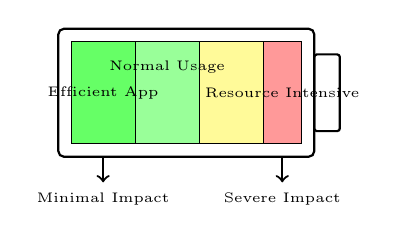
\begin{tikzpicture}[scale=0.65]
					% Battery outline
					\draw[rounded corners=2pt, thick] (0,0) rectangle (5,2.5);
					\draw[rounded corners=1pt, thick] (5,0.5) rectangle (5.5,2);
					
					% Battery segments
					\draw[fill=green!60] (0.25,0.25) rectangle (1.5,2.25);
					\draw[fill=green!40] (1.5,0.25) rectangle (2.75,2.25);
					\draw[fill=yellow!40] (2.75,0.25) rectangle (4,2.25);
					\draw[fill=red!40] (4,0.25) rectangle (4.75,2.25);
					
					% Resource impacts
					\node[align=center] at (0.875,1.25) {\tiny{Efficient App}};
					\node[align=center] at (2.125,1.75) {\tiny{Normal Usage}};
					\node[align=center] at (4.375,1.25) {\tiny{Resource Intensive}};
					
					% Impact arrows
					\draw[->, thick] (0.875,0) -- (0.875,-0.5) node[below, align=center] {\tiny{Minimal Impact}};
					\draw[->, thick] (4.375,0) -- (4.375,-0.5) node[below, align=center] {\tiny{Severe Impact}};
				\end{tikzpicture}
			}
		\end{center}
		
	\end{frame}
	
	\begin{frame}
		\frametitle{Offline Functionality: Making Apps Work Without Internet}
		
		\begin{itemize}
			\item \textbf{Offline functionality} allows apps to remain useful when internet connectivity is unavailable, slow, or unreliable—a common scenario for mobile users on the move.
			\item Implementing offline capabilities typically involves \textbf{local data storage} using technologies like SQLite databases, key-value stores, or file system caching to retain essential information on the device.
			\item Effective offline apps use \textbf{synchronization strategies} to reconcile local changes with remote data when connectivity is restored, handling potential conflicts and data merging intelligently.
		\end{itemize}
		
		\begin{block}{\scriptsize{Offline Implementation Approaches}}
			\scriptsize{
				\begin{tabular}{|p{2.5cm}|p{5.5cm}|}
					\hline
					\textbf{Approach} & \textbf{Best For} \\
					\hline
					Full offline mode & Travel apps, field work tools, rural areas \\
					\hline
					Cached content & News apps, reference materials, catalogs \\
					\hline
					Offline data entry & Forms, surveys, note-taking applications \\
					\hline
					Progressive loading & Social media, content-heavy applications \\
					\hline
				\end{tabular}
			}
		\end{block}
		
	\end{frame}
	
	\begin{frame}
		\frametitle{Security Fundamentals: Protecting User Data on Mobile}
		
		\begin{itemize}
			\item Mobile apps often handle sensitive user information, making security a critical concern—according to industry reports, over 85\% of mobile apps have security vulnerabilities that could lead to data breaches.
			\item \textbf{Secure data storage} is essential, with sensitive information encrypted both in transit (using HTTPS/TLS) and at rest (using platform-appropriate encryption APIs).
			\item \textbf{Authentication and authorization} must be implemented carefully, with secure practices for password handling, multi-factor authentication when appropriate, and proper session management.
			\item Mobile apps should follow the principle of \textbf{least privilege}, requesting only the permissions absolutely necessary for functionality and handling granted permissions responsibly.
		\end{itemize}
	\end{frame}
	
	\begin{frame}
		\frametitle{Accessibility in Mobile Apps: Designing for All Users}
		
		\begin{itemize}
			\item \textbf{Accessibility} refers to designing apps that can be used by everyone, including people with disabilities such as visual impairments, hearing limitations, motor difficulties, or cognitive challenges.
			\item Approximately 15\% of the global population lives with some form of disability, making accessibility not just an ethical consideration but also an important factor for reaching a broader audience.
			\item Beyond compliance with regulations like the ADA or WCAG guidelines, accessible design often improves usability for all users, especially in challenging contexts like bright sunlight or noisy environments.
		\end{itemize}
		
		\begin{block}{\scriptsize{Key Accessibility Considerations}}
			\scriptsize{
				\begin{itemize}
					\item \textbf{Adequate contrast:} Ensure text and interactive elements have sufficient contrast against backgrounds
					\item \textbf{Adjustable text size:} Support system font scaling without breaking layouts
					\item \textbf{Touch target size:} Make interactive elements at least 44×44 points for easy tapping
					\item \textbf{Alternative input methods:} Support voice control and external hardware like keyboards
					\item \textbf{Meaningful labels:} Provide descriptive labels for screen readers to announce
				\end{itemize}
			}
		\end{block}
		
	\end{frame}
	
	\begin{frame}
		\frametitle{Mobile App Testing: Ensuring Quality Across Devices}
		
		\begin{itemize}
			\item Mobile app testing is particularly challenging due to the \textbf{fragmentation} of devices, screen sizes, operating system versions, and hardware capabilities across the user base.
			\item \textbf{Automated testing} is essential for mobile applications, with unit tests verifying individual components, integration tests checking component interactions, and UI tests validating the complete user experience.
			\item \textbf{Real device testing} remains critical despite the availability of simulators and emulators, as only physical devices accurately represent real-world conditions including touch sensitivity, performance constraints, and sensor behavior.
			\item Testing should incorporate different network conditions (\textbf{connection testing}) to ensure the app behaves appropriately on fast WiFi, slow cellular connections, and when transitioning between connectivity states.
		\end{itemize}
	\end{frame}
	
	\begin{frame}
		\frametitle{Testing Pyramind}
		\begin{center}
			\scriptsize{
				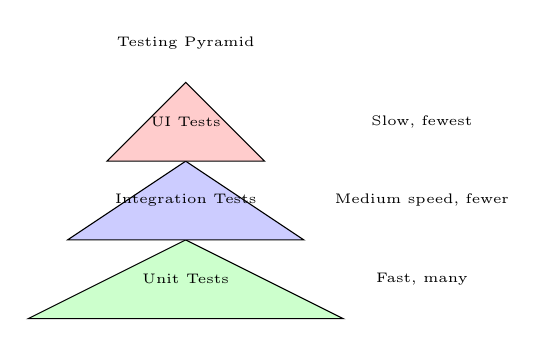
\begin{tikzpicture}[very node/.style={rectangle, rounded corners, draw, align=center}]
					% Testing pyramid
					\filldraw[fill=green!20] (0,0) -- (4,0) -- (2,1) -- cycle;
					\filldraw[fill=blue!20] (0.5,1) -- (3.5,1) -- (2,2) -- cycle;
					\filldraw[fill=red!20] (1,2) -- (3,2) -- (2,3) -- cycle;
					
					% Labels
					\node[draw=none] at (2,0.5) {\tiny{Unit Tests}};
					\node[draw=none] at (2,1.5) {\tiny{Integration Tests}};
					\node[draw=none] at (2,2.5) {\tiny{UI Tests}};
					
					% Stats
					\node[draw=none] at (5,0.5) {\tiny{Fast, many}};
					\node[draw=none] at (5,1.5) {\tiny{Medium speed, fewer}};
					\node[draw=none] at (5,2.5) {\tiny{Slow, fewest}};
					
					% Title
					\node[draw=none] at (2,3.5) {\tiny{Testing Pyramid}};
				\end{tikzpicture}
			}
		\end{center}
		
	\end{frame}

\end{document}